%%%%%%%%%%%%%%%%%%%%%% Version Information %%%%%%%%%%%%%%%%%%%%%%%%%%% 
% This LaTeX2e thesis template is based on the nuthesis-template
% provided by Miguel A. Lerma. It was renamed and edited to meet the
% requirements given in the Thesis-Dissertation Instructions of the
% School of Graduate Studies of Case Western Reserve University by
% Initial Version: Frank Ernst (Dr. rer. nat. habil., Professor). 
%   Version dated 2006-08-23.
% Latest Version: Roger French (Professor). 
%  SDLE Center Authors: Nicholas Wheeler, Myles Murray, Heather Lemire
%  Version dated 2015
%%%%%%%%%%%%%%%%%%%%%%%%%%%%%%%%%%%%%%%%%%%%%%%%%%%%%%%%%%%%%%%%%%%%%% 

%%%%%%%%%%%%%%%%%%%%%%%%%%%%%% DISCLAIMER %%%%%%%%%%%%%%%%%%%%%%%%%%%%
% The author of the thesis remains responsible for fulfilling all
% requirements.
%%%%%%%%%%%%%%%%%%%%%%%%%%%%%%%%%%%%%%%%%%%%%%%%%%%%%%%%%%%%%%%%%%%%%%

%%%%%%%%%%%%%%%%%%%%%%%%%%%%% DESCRIPTION %%%%%%%%%%%%%%%%%%%%%%%%%%%%
% cwru-cse-thesis.tex is the master file that compiles the whole thesis.
% Individual chapter files located in 'content' folder
% Appendix files located in 'app' folder
% bibtex file for references located in 'refs' folder
% figure files go in the 'figs' folder
% the 'input' folder has style files for tex compiling
%%%%%%%%%%%%%%%%%%%%%%%%%%%%%%%%%%%%%%%%%%%%%%%%%%%%%%%%%%%%%%%%%%%%%%

\documentclass[help,12pt,onepage,reqno]{input/CWRU-Thesis}

% Uncomment *one* of the following lines if you are tired of TeX's
% Computer Modern fonts:
\usepackage{fourier} 
%\usepackage{mathpazo}
%\usepackage{mathptmx}

% Graphics.
\usepackage[pdftex]{graphicx}
\usepackage{subfig}
\usepackage{pdflscape} % landscape environment
%\usepackage{subfigure}
\usepackage{longtable}
\usepackage{float}
\newtheorem{definition}{Definition}
\newtheorem{theorem}{Theorem}
\newtheorem{lemma}{Lemma}
\newtheorem{corollary}{Corollary}
\newtheorem{prop}{Proposition}
% The following makes graphicx work with pdf and jpg files. Files with
% same names and different extensions will be recognized in sequential
% order.
\DeclareGraphicsExtensions{.jpg, .pdf} 
\newcommand{\vect}[1]{\mathbf{#1}}
% PDFPages imports entire PDF pages.
%\usepackage[draft]{pdfpages} % not sure that this actually works
\usepackage[final]{pdfpages}
\usepackage{natbib}

% Sets pdftex to included versions up to 1.6
%\pdfminorversion=6
\pdfoptionpdfminorversion=6

% Chapterbib enables separate bibliographies after each chapter.
%\usepackage[sectionbib]{chapterbib}
%\usepackage[rootbib]{chapterbib}

\usepackage{verbatim} %for comment environment
\usepackage{listings}
% % to allow underscore in text, doesn't work if you actually use
% % underscores in the latex doc
% \usepackage{underscore}
% \begingroup
%   \lccode`\~=`\_
% \lowercase{\endgroup
%   \pdfstringdefDisableCommands{\let~\relax}%
% }

% Wrapfig wraps tables and figures.
\usepackage{wrapfig} 
\usepackage{multirow}

% footnotes in tables
\usepackage{threeparttable}
% \usepackage{footnote}
% \makesavenoteenv{tabular} % makes tables handle footnotes correctly

% Your packages can go here:
\usepackage{input/KL-Typing-Aids}

% Author and title
\author{\uppercase{Boning Zhao}}
\title{A THEORETIC APPROACH FOR BINARY GAME TREE EVALUATION}

\degree{Master of Science}  
% Default: Doctor of Philosophy.

\adviser{Vincenzo Liberatore}     
% Optional -- Default: Empty.

\department{Electrical Engineer and Computer Science}     
% No Default.

\graduationmonth{Dec}      
% The default is January, May, or August depending on current date.

\graduationyear{2019}
% Default: current year.
% CAUTION: next January could be *next* year.


%\includeonly{05-Background, 06-Methods}
% Use \includeonly to select the chapters to include if you are using
% the \include command below. This way you can latex only a the part
% you are working on, which is faster than latexing the entire thesis.

% Margin kerning.
\input input/protcode.tex

%	%------------------- Markup
	% new commands for markup/editing purposes
	% make a \newcommand for your self, this rhf set is for Roger (rhf) and Dan (dmd)
	\usepackage{xcolor}
	\usepackage{ulem}
		% color names = red, green, blue, cyan, magenta, yellow, black, gray, white,  
		%   darkgray, lightgray, brown, lime, olive, orange, pink,  purple, teal, violet
		%   
			%-------------------------
				% rhf = Roger markup
			\newcommand{\rhf}{\textcolor{red}} % for rhf = Roger is red text
			\newcommand{\rhfcomm}[1]{
			       \colorbox{yellow}{#1} % Roger is yellow highlight
			       }
			\newcommand{\rhfstr}[1]{
				\sout{#1} %Roger's strikethrough
			}
			%-------------------------
			
\usepackage{hyperref} % enables hyper links in the document's pdf file output

\begin{document}%%%%%%%%%%%%%%%%%%%%%%%%%%%%%%%%

%Margin kerning.
\setprotcode \font
{\it \setprotcode \font}
{\bf \setprotcode \font}
{\bf \it \setprotcode \font}

% % To turn off hyphen protrusion at end of line, set to "0".
\pdfprotrudechars=1 

\frontmatter
%\pagenumbering{roman}

% Title page.
\maketitle		

% Page for signatures of the committee members.
%For the final turn in, you do not need this page signed, just dated.
% to date this page, cludgy way to do it is replace Signature/Date with the Date
%Found in the CWRU-thesis.cls file, line 327
\signaturepage
{Dr. Vincenzo Liberatore}\newline
\newline
{Date: December 2, 2019}
%\sign{\fe}{Member}{\dmse} %if pre programed can use short name thing

% Copyright page. You do not need a copyright page unless
% you are applying for a copyright.
%\copyrightpage 

% Dedication page (optional). Please indicate linebreaks by "\\".
\dedication{Dedicated to *your\\dedication message goes here*}

% Preface (optional).
%\preface
%\input{03-Preface}

% Table of Contents will be automatically generated and placed here.
\tableofcontents
% List of Tables and List of Figures will be automatically generated
% and placed here.	
%\subfiglabelskip=0pt % suppresses spacing after empty subfiglabel set
                     % to 0pt; for use with subfigure.sty
\listoffigures		

% Acknowledgements (optional).
\acknowledgements
\begin{sloppypar}
Above all I would like to thank my advisor, Professor Vincenzo Liberatre, for his assistance through the entire process of
creating this thesis topic and finishing this research. At the beginning of this thesis I knew very little of the process of research, but Professor Liberatre provided advice and suggestion which helped me find a way to begin the experiment. Whenever I met problems, he guided me to out of stuck with patience. It is impossible to complete this thesis without him.

I also would like to express my thanks to my parents. During my first 24 years of life, they tried their best to support my life and study, and I even didn't acknowledge this for a long time. Their love and support is the reason I could be here. 


\end{sloppypar}

% Abstracts must not exceed 350 words in dissertations and 150
% words in other theses.
\abstract
\begin{sloppypar}
 The Binary Decision tree model is perhaps the simplest model that computes Boolean functions: it charges only for reading an input variable. We proposed a theoretical binary game tree evaluation analysis process which could provide better lower bound compared with lower bound provided by previous analysis. Based on the concept of reluctant input, We study the power of randomness in this model with both directional and non-directional algorithm, and made the comparison of their efficiency with lower bound. These results are obtained via general and efficient methods for computing  lower bounds on the probabilistic complexity and based on a special type of uniform binary decision tree, which we call it NOR-tree, which is an equivalent transformation of AND/OR tree. As a result of study, we finally build up a more accurate analysis process. In order to test its versatility, we also apply this analysis process to two different types of binary game tree: Fibonacci tree and skew-F tree. Both of these two have more complicated structure for game tree evaluation. The results shows that this process could also be used for getting other type of game trees lower bound.

\newpage
\end{sloppypar}
%can you run bibliography on abstract?
%\bibliographystyle{plainnat}
%\bibliography{my_references}
 

\mainmatter             
\pagenumbering{arabic} 

% Change hyperlink color to a bluish hue that is fairly visible, but
% not disturbing in long lists of references, and will also print well
% in black and white. Up to this point, the hyperlink color was black
% (default) to avoid that the tables of contents, figures, and tables
% entirely appear in color.
\definecolor{felinkcolor}{rgb}{0,0,0.5}

\chapter{Introduction}

 Game tree is defined as a rooted tree whose internal nodes at even distance from the root are labeled MIN and those at odd distance are labeled MAX.\cite{GT} Each leaf of a game tree is real number which called value. We evaluate the game tree by the following step: Every leaf return its value; Then every MIN node returns the smallest value by its children and the MAX node returns the largest. The aim of the evaluation process is to determine the root's value.

 The evaluation of game trees is a central part in artificial intelligence and game theory,especially in game-playing programs. The children of a node means the options available to one or two players in a game. The leaves of a game tree represent the value of the game for one or two players. One player seeks to maximize this value, and another will try to minimize it. \cite{MCS}For evaluation process, the algorithm will choose a leaf and reads its value. The number of this steps taken by an algorithm is the only issue we focus on, which means no other computation will be charged for the algorithm.
 
 This thesis will be limited in binary tree, whose leaves value is 0 or 1. Therefore, we can transform each MAX node to Boolean OR operation and MIN node to Boolean AND operation, which leads the analysis on AND-OR tree.Furthermore, We investigate a simple model called Nor-tree for computation of Boolean functions. It is a binary boolean decision tree which is a transformation is equivalent AND/OR tree with even height,which will be introduced in following section. 
 
 For instance, a uniform tree whose node has $n$ children and all leaves are at distance $k$ from the root. The evaluation of this game tree is to study the maximum number of steps to evaluate all instances of the game tree in same height and with same leaves. this problem consists of the trees structure and Boolean value of $n^k$ leaves.
 
 There are two ways to evaluate game tree: deterministic algorithm and randomized algorithm. For deterministic algorithm, the choice of the next step is a deterministic function of the values at the leaves read so far. For any deterministic function, there exists an instance that needs to read all the leaves. Therefore, the evaluating result for a deterministic algorithm is always $n^k$. \cite{DETER}
 
 A randomized algorithm is an algorithm which contains randomness as part of its logic. For game tree evaluation, a randomized algorithm means the choice of the next leaf to be read may be randomized. Using randomized algorithm is to achieve good performance in the "average" cases over all possible instances.\cite{RG} We will focus on randomized algorithm in this thesis, because randomized algorithm could benefit game tree evaluation compared with deterministic algorithm. A simple example, For a binary tree with height $k$. Any deterministic algorithm will have to evaluate all $2^k$ leaves. 
 
 A simple randomized algorithm which will take the probability $p<1$ to choose which step to read. For AND node return 0, if a deterministic algorithm reads the 0 at second step, a randomized algorithm will have probability $p$ to read it in the first step, then we don't need to visit the other one. Its expected number of step is $2-p$ which is less than $2$. Similarly, for OR node, if it returns 1, the expected number for randomized algorithm is $2-p$. This adversary could be used for proving the randomized algorithm works better than deterministic algorithm in evaluating game tree, which we will show in section 2.
 
 In this thesis, we proposed a game tree evaluation process compared with the one in "Randomized Algorithm", in which the proof has some loose and the lower bound is not tight. \cite{RANDOM1995} The game tree evaluation process is based on the game theory and Yao's Principle\cite{YAO}. This process provide better lower bound analysis and could be expanded to evaluating not only uniform binary tree but also other types binary game tree.

 In chapter 2, we provide background information of game tree, minimax algorithm and randomized algorithm, which are important for understanding the following analysis. We also introduce basic evaluation steps for nor-tree, a binary tree which equivalent to AND-OR tree. In chapter 3, we discuss the analysis of directional algorithm's and its lower bound on Nor-tree. In chapter 4, we  present the lower bound proof for non-directional algorithm, which includes three different cases. We also make a comparison between directional algorithm and non-directional in order to find which is better. In chapter 5, we will introduce two different binary game tree, skew-F tree and Fibonacci tree, and show whether this game tree evaluation process could also be used for evaluating them. This step is to test versatility of this analysis process.  In chapter 6, we conclude by describing the whole process and future work using this method.


%\bibliographystyle{plainnat}
%\markright{\textit{Bibliography}}
%\renewcommand{\chaptername}{}
%x\bibliography{KL-Thesis}

\vfill


%background
\chapter{Background and Definition} 

%\label{ch:bg}
In this chapter, we will introduce some background of the algorithm and theory, which we used in the following research and proof. This part includes: benefit of randomized algorithm in game tree evaluation, minimax principle, Nor-tree definition and proof of its equivalence with AND-OR tree, Nor-tree evaluation process, reluctant input, which are all important in our research.


\section{Background}
\subsection{Benefit of Randomized Algorithm}
In previous chapter, we showed that randomized algorithm will have better expected number in evaluating compared with deterministic algorithm in some situation. We will prove this by induction. For an AND-OR tree $T$ with height $2k$(denoted as $T_{2k}$), the expected number for deterministic algorithm is $4^k$, now we argue that for the randomized algorithm we mentioned before the expected cost is at most $3^k$.

The basis condition when $k = 1$ just follows the analysis we made in chapter 1. Then we assume that for $T_{2k-1}$ the expected number needs to be read is $3^{k-1}$. Then by induction, we firstly analyze a tree with an AND node as root. If the root evaluates to 1, then both of its children at OR node return 1. The expected cost of this situation is $2 \times 3^{k-1}$, because both of the children need to be evaluated. On opposite, if the root evaluates to 0, the with probability $\frac{1}{2}$ the $0$ node will be choose first, then the expected cost is $\frac{1}{2} \times 3^{k-1}$. Other side, with $\frac{1}{2}$ probability the 0 one will be visit in second step, then $2\times \frac{1}{2} \times 3^{k-1}$. Then putting these two result together, we could determine the expected cost of this AND-OR tree is
\begin{equation}
	\frac{1}{2} \times 3^{k-1}+2\times \frac{1}{2} \times 3^{k-1}=\frac{3^k}{2}
\end{equation}
Similarly, we could also get root node is an OR node has the same expected cost. Therefore we could see that randomized algorithm is better than deterministic algorithm in game tree evaluating.  

\subsection{Minimax Principle}
Minimax Algorithm is widely used in decision making and game theory in order to find the optimal move for a specific player. The minimax principle is the only known general technique for proving lower bounds of randomized algorithms. It only could be applied to algorithms those could finish in finite time. In minimax algorithm, we assuming that both the player and his opponent play optimally. There is an example for illustrating the basic method of it:

\begin{figure}[H]
	\centering
	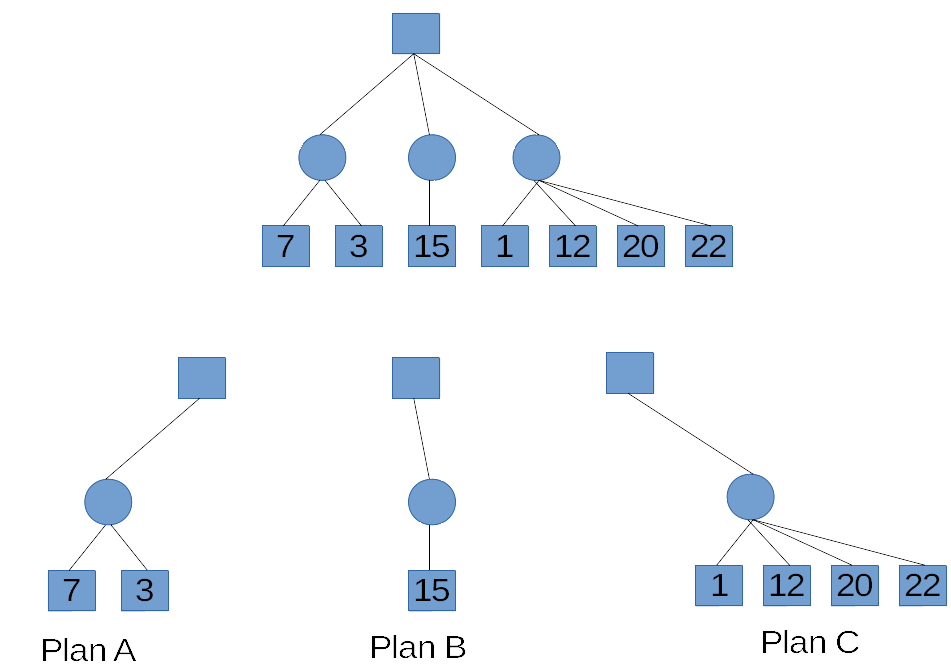
\includegraphics[width=0.5\linewidth]{minimax0}
	\caption{example of minimax principle}
	\label{fig:minimax0}
\end{figure}
Let square be player A ,and circle representing player B. Each leaf represents a possible benefit for player A. The aim of this game is for B to minimize A's benefit and A will try to maximize his benefit. If player A choose Plan A, then player B has two choices, in order to minimize player A's benefit. B will choose 3. For Plan B, player B has no choices but to let player A get 15. At last if plan C is chosen, then  player A could only get 1 benefit. Therefore in order to maximize his benefit, player A will choose plan B.

In order to understand the minimax principle theoretically. We will introduce some basic concept in game theory. One important concept is two-person zero-sum game, in which minimax principle could be applied. Let's say there are two player T and F. They will choose from three tarot card: Fool, Justice, Judgement. They don't know what card the opposite choose. Then they will show the card at the same time. The winner is determined by the following rules: The Fool beats Justice and wins 5 dollar; Justice wins the Judgement and Judgement will beat the Fool. Both of this two cases wins 3 dollar.If they choose the same card, then it comes to a draw. The game described above os an instance of a two-person zero-sum game. A two-person zero-sum game always could be represented as a payoff matrix. Like the game above could be:
\begin{table}[H]
	\caption{Matrix for tarot game}
	\begin{tabular}{lccc}
		\hline
		\hline
		  T $\backslash$ F & Fool & Justice & Judgement \\
		  \hline
		  \hline
		  Fool & 0 & 5 & -3\\
		  \hline
		  Justice & -5 & 0 & 3\\
		  \hline
		  Judgement & 3 & -3 & 0\\
		 \hline
		 \hline
	\end{tabular}
\end{table}

Let's set the matrix as $M$. Every row could denote the strategy chosen by player T and every column could be the strategy for player F.Then the entry $M_{ij}$ is the amount paid from T to F when T chooses strategy $i$ and F chooses $j$. Therefore, F will try to minimize the payoff and T will try to maximize the payoff. Because both player T and F has no idea about what strategy their opponent will choose. If T choose strategy $i$, then the payoff will be $min_jM_{ij}$ and no matter what F will choose the payoff is guaranteed. We could see the optimal strategy for player T is to maximize $min_jM_{ij}$.Similarly, We could get the player F's optimal payoff is $min_jmax_iM_{ij}$. For all payoff matrices we have:
\begin{lemma}
	$max_imin_jM_{ij} \le min_jmax_iM_{ij}$
\end{lemma}  
When the equality exists, which mean the game is said has a solution and the value of the game is the equal to the lower bound of payoff from player trying to maximize it or the upper bound of payoff from player trying to minimize it. The solution also could be called as saddle point\cite{SA}. However, not all games have a solution under this type strategy. Like in tarot game, Value for T is 3 and F is -3. Both of the player will try to improve their payoff as much as possible. So far we discussed is about pure or deterministic strategy. In order to solve the game has no solutions, we should use strategies with randomization in it, which are called mixed or randomized strategies. A randomized strategy is a probability distribution on the set of all possible strategies. For example, in tarot game(Let's say payoff matrix $M$ has m rows and n columns), player T will have probability $p_i$ to choose row $i$ as his strategy and the randomized strategy for T is a vector $\vect{p} = (p_1,...,p_n)$. Similarly, let's define randomized strategy for F as $\vect{q} = (q_1,...,q_m)$, which denotes the probability distribution on columns. Therefore we could get the expectation payoff as:
$$ E[pay] = p^TMq = \sum_{i=1}^{n}\sum_{j=1}^{m}p_iM_ijq_j$$   
Similarly to how we analyze deterministic strategy, we could get The optimal lower bound for player T is $L = max_pmin_qp^TMq$ and optimal upper bound for player F is $U=min_qmax_pp^TMq$. Then here comes a well-known Minimax Theorem of von Neumann\cite{VON}.For any two-person zero-sum game specified by a payoff matrix M:
\begin{theorem}
	$max_{\vect{p}}min_{\vect{q}}\vect{p}^TM\vect{q} = min_{\vect{q}}max_{\vect{p}}\vect{p}^TM\vect{q}$
\end{theorem}
which means that this type of game always has a solution and a pair of randomized strategies ($\vect{p}$,$\vect{q}$), which helps reach the solution is the saddle point of the game. We also could easily find that $\vect{p}^TM\vect{q}$ is a linear function of $\vect{q}$ and it could be simplified by setting 1 to the smallest coefficient $q_j$ and 0 to others. We could find that if player F knows the probability distribution $\vect{p}$, then his optimal solution will be a deterministic strategy. The theorem 1 also could be lead to a simplified version which invented by Loomis\cite{LOOMIS}:
\begin{theorem}
		$max_{\vect{p}}min_{j}\vect{p}^TMu_j = min_{\vect{q}}max_{i}e_{i}^{T}M\vect{q}$ (where $u_i$ means a unit vector with a 1 in i position and 0s in others)
\end{theorem}
\subsection{Yao's Principle}
Yao's principle, which also called 'minimax principle' claims that the expected cost of randomized algorithm on the worst-case input is no better than the expected cost for a worst-case probability distribution on the inputs of the deterministic algorithm that performs best against that distribution.\cite{YAO} Let's use the tarot game in previous game to illustrate this. We set player F as the one who apply the algorithm(every column), and player T as adversary choose the input(every row).Let's say the payoff from player F to player T is the valuable cost of the performance of an algorithm with rows as a finite set of all possible inputs and columns as a finite set of possible deterministic algorithms that always produces a correct solution. Clearly, player F will choose an algorithm which minimizes the payoff, and the  player T will try to maximize it.

In this problem, we could observe that the number of distinct inputs is equal to the number of distinct deterministic algorithms which could promise finish with correct solution. A deterministic strategy for player T is an input and for player F is a deterministic algorithm. A randomized strategy for T is a distribution over all inputs and a randomized strategy for F is a distribution over the space of deterministic algorithms\cite{M}. We could see this is a Las Vegas randomized algorithm\cite{LAS}. Let's set $L_F$ is the worst case algorithm cost for all deterministic algorithm and $U_T$ is the best case algorithm cost for the worst deterministic algorithm choice. We denote $L_F$ as the deterministic complexity for the game and $U_T$ as the randomized complexity \cite{S}. In this thesis, we will focus on complexity which is the expected algorithm cost of the best deterministic algorithm with worst distribution on input\cite{MT}. This  complexity is smaller than deterministic one because the algorithm knows the distribution.\cite{YAOC}

From Loomis Minimax Principle, we could get the complexity equals the least possible costs with any randomized algorithm. Now we could apply the Minimax Principle as:
Let $G$ be a two-person zero-sum game problem. It has a finite set $\vect{I}$ as input and a finite set $\vect{D}$ as the set of all possible, always correct deterministic algorithms. For instance I $\in \vect{I}$ and D $\in \vect{D}$, we denote C(I,D) as the cost for deterministic algorithm over input I. The probability distributions on $\vect{I}$ and $\vect{D}$ are $\vect{p}$ and $\vect{q}$. Then we could get theorem 1 and 2 as :
\begin{equation}
   max_{\vect{p}}min_{\vect{q}}E[C(\vect{I}_{\vect{p}},\vect{D}_{\vect{q}})] = min_{\vect{q}}max_{\vect{p}}E[C(\vect{I}_{\vect{p}},\vect{D}_{\vect{q}})]
\end{equation}

\begin{equation}
max_{\vect{p}}min_{D\in\vect{D}}E[C(\vect{I}_{\vect{p}},\vect{D})] = min_{\vect{q}}max_{I\in\vect{I}}E[C(I,\vect{D}_{\vect{q}})]
\end{equation}

Then the Yao's Minimax Principle comes:
\begin{theorem}
	$$min_{D\in\vect{D}}E[C(\vect{i}_{\vect{p}},D)] \le max_{I\in \vect{I}}E[C(I,\vect{D}_{\vect{q}})]$$
\end{theorem}

Yao's Principle is a very useful tool for proving the lower bound for randomized algorithm. It claims the expected cost of the optimal deterministic algorithm for a randomized chosen input distribution is the lower bound for the cost of optimal randomized algorithm for problem. The reduction to a lower bound on deterministic algorithms makes Yao's principle is very powerful in proving lower bound.\cite{YAOS}

\subsection{Nor-Tree Evaluation}
In previous chapter. We introduce the binary tree evaluation could be transformed to an AND-OR tree evaluation by limited the leaves value with in 0 and 1. In this thesis, we will use a more simplified tree model which called nor-tree, its logic is following:
\begin{figure}[H]
	\centering
	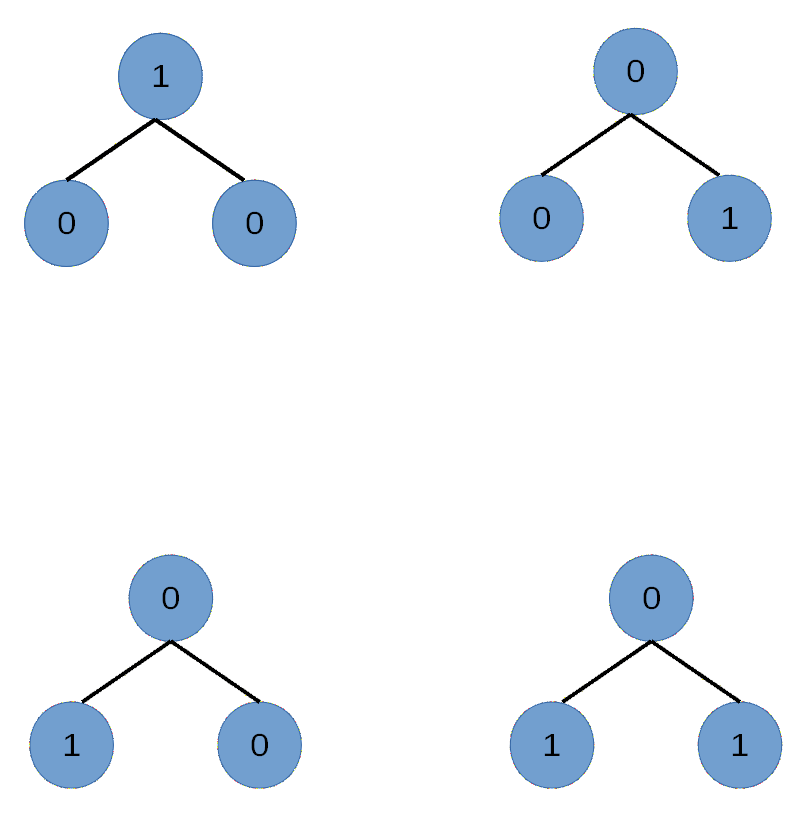
\includegraphics[width=0.5\linewidth]{Nortree}
	\caption{Nortree logic}
	\label{fig:nortree}
\end{figure}
A balanced binary tree whose all leaves are at the distance 2k from root is equal to the same structure nor-tree. Firstly, we already proved that this is equivalent to the same height AND-OR tree. Then Let's see when k = 1. Let's denote the 4 notes as a,b,c,d. The value of the root of AND-OR tree is $(a \bigvee b) \bigcap(c \bigvee d)$ and the nor-tree's is $\neg(a \bigvee b) \bigcap \neg (c \bigvee d)$. We could see this two is equal. Assuming that k=n-1 this claim is correct. Similarly, we could prove when k=n, this is also correct.
\begin{figure}[H]
	\centering
	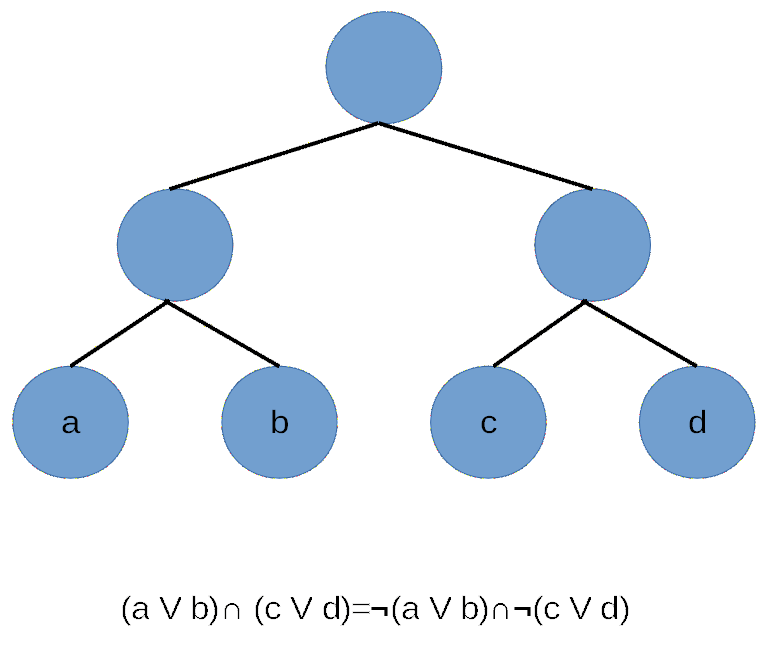
\includegraphics[width=0.5\linewidth]{ao_nor}
	\caption{AND/OR tree equivalent to Nor-tree with Same Height }
	\label{fig:aonor}
\end{figure}

Then for the evaluation of this nor-tree we have:
$$ h(x)=\left\{
\begin{aligned}
&h_{left}(x_L) + h_{right}(x_R) & if\ algorithm=L\ and\ left\ equals\ to\ 0\\
&h_{left}(x_L)  & if\ algorithm=L\ and\  left\ equals\ to\ 1\\
&h_{left}(x_L) + h_{right}(x_R) & if\ algorithm=R\ and\ right\ equals\ to\ 0\\
&h_{right}(x_R) & if\ algorithm=R\ and\ right\ equals\ to\ 1
\end{aligned}
\right.
$$
which could be described as:
\begin{lstlisting}[title=evaluation of nor-tree, frame=shadowboc]
1:NorEvaluation(node)
2:if (node.type = "LEAF") then
3:   return(node.value)
4:end if
5:if (node.type = "Nor") then
6:  Toss a coin
7:  if (Heads) then
8:  p1 = NorEvaluation(node.left)
9:  if(p1 = 1) then 
10:   return 0
11:  else
12:  p2= NorEvaluation(node.right) 	
13:    if(p2 = 0)
14:      return 1
15:    else
16:      return 0;
17:    end if
18:  end if
19:end if
\end{lstlisting}
Yao's principle has its flexibility in the choice of input distribution. In "Randomized Algorithm", the author just choose the distribution by arbitrary and ignored conditional probability in internal nodes. By experiments simulates the leaves value distribution with algorithm we find that the algorithm does not effect the best payoff of the tree, and we could find the pattern of the optimal nor-tree is:
\begin{enumerate}
	\item The value of the root is always 1.
	\item When the value of node equals to 0, the value of two leaves will has 1/2 probability to be (0,1) and 1/2 to be (1,0);
\end{enumerate}

In this thesis, we will use L(k,i) to denote the min expected leaves visited by algorithm of node 
in k level whose value is i(payoff for a tree of height k, its value is i, and k is even).

\section{Definitions}
We define the value of a leaf as its input value (leaf label), and 
the value of an internal node as true if both children are false,
and false otherwise.
We define
 an algorithm for a NOR tree $T$ as a process to find a specific ordering $\sigma$ of 
$T$'s leaves. It always starts with a leaves ordering. Based on the value of the vertices's already been determined, it will rearrange the ordering in order to determine the root's value by visiting as less leaves as possible. 

The prefix of $\sigma$ of length $t$ will be denoted as $\sigma_t$.
Given a leaf labeling and an ordering $\sigma$, 
we associate a logical time-stamp to each tree vertex as follows.
We will say that a leaf $u$ is evaluated at time $t$ 
if $\sigma_t$ is the shortest prefix of $\sigma$ containing $u$.
It is immediate to see that $u$ is evaluated at time $t$ if and only if
the $t$th element of $\sigma$ is $u$.
If $u$ is an internal node whose value is false,
we will say that $u$ is evaluated at time $t$ if 
$\sigma_t$ is the shortest prefix such that both children of $u$
have been evaluated at time $t$ or earlier. 
Conversely, if $u$ is an internal node whose value is true,
$u$ is evaluated at time $t$ if 
$\sigma_t$ is the shortest prefix such that at least one
child of $u$ whose value is false 
has been evaluated at time $t$ or earlier.
Intuitively, the definition captures the idea that the value of an 
internal node becomes available as soon as there is the minimum
amount of information needed to evaluate it. 
We define the  cost of a NOR tree algorithm
as the time at which the root is evaluated.
Note that once the root is evaluated, 
the remaining suffix of $\sigma$ is irrelevant to 
$\sigma$'s cost. 
In light of this observation, we will say that 
$\sigma$ omits leaf $u$ if leaf $u$ appears after
the root has been evaluated.
Similarly, we say that $\sigma'$ omits an internal node $x$ 
if node $x$ appears after the root has been determined.

Note that any tree traversal implicitly defines a 
leaf ordering $\sigma$ as the subsequence of the traversal order
containing only the leaves. 
Conversely, given a leaf ordering $\sigma'$, we define its 
canonical traversal as the vertex ordering whose leaf 
subsequence is $\sigma'$,
where a true internal node $u$ appears at the earliest point after
both of its children, and
where a false internal node $u$ appears at the earliest point after
one of its true children.
It is immediate to see that the evaluation order of $\sigma$ can be 
reconstructed from its canonical traversal. 

\begin{figure}[H]
	\centering
	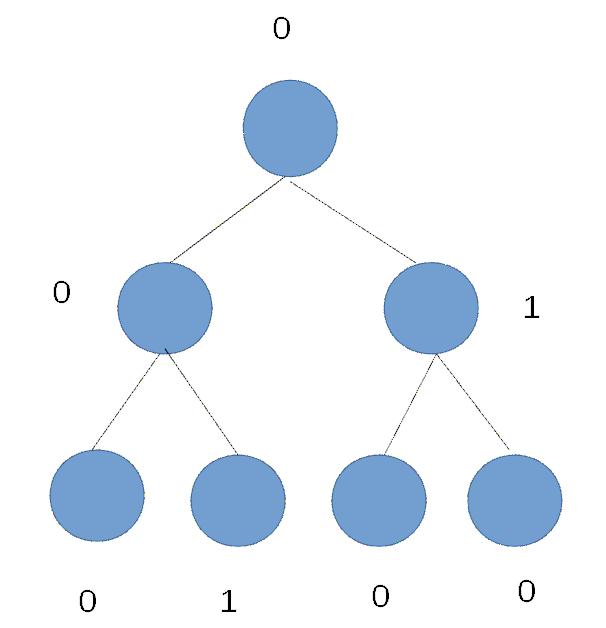
\includegraphics[width=0.3\linewidth]{def_0}
	\caption{A NOR-tree of height 2 with a binary labeling of the leaves
		and calculated values in the internal nodes.}
	\label{fig:def0}
\end{figure}
Figure \ref{fig:def0} shows an example of these definitions.
Suppose that an algorithm visits the four leaves from left to right.
Then, the corresponding leaf ordering is $\sigma' = (a, b, c, d)$.
The canonical ordering $\sigma$ can be constructed as follows.
First, since $\sigma'$ is a subsequence of $\sigma$, then
the leaves appear in the order $a, b, c, d$ within $\sigma$
Since $e$ is a false internal node, node $e$ appears in $\sigma'$
immediately after its true child $a$. 
Since $f$ is a true internal node, node $f$ appears in $\sigma'$ immediately
after $c$ and $d$. 
Finally, since $g$ is false, node $g$ appears in $\sigma'$ immediately
after $f$.
By putting these constraints together, we obtain that 
$\sigma' = (a, e, b, c, d, f, g)$.
It is immediate to see that a better algorithm would visit only three leaves
if $\sigma_3 = (a, c, d, b)$ and $\sigma'_3 = (a, e, c, d, f, g, b)$.
and that the optimal visit enables the tree evaluation by visiting
only the leaves $c$ and $d$ with 
$\sigma_2 = (c, d, a, b)$ and $\sigma'_2 = (c, d, f, g, a, e, b)$.
Note that the algorithm $\sigma_2$ omits the leaves $a$ and $b$.


%\bibliographystyle{plainnat}				%Uncomment this if you want a bibliography on each chapter
%\markright{\textit{Bibliography}}
%\renewcommand{\chaptername}{}
%\bibliography{my_references}

%\vfill


%Directional part
\chapter{Analysis of Directional Algorithm}
In this chapter, we will analyze the process of deterministic directional algorithm for nor-tree evaluation. With computing the lower bound of this algorithm, we will compare its difference with general evaluation process.
%\label{ch:bg}

\section{Directional Algorithm}
We begin by analyzing a class of directional algorithms' lower bounds, as per the following definition.
	\begin{definition}
	\label{def:directional}
	A {\em deterministic directional algorithm\/} 
	for a NOR tree $T$ is the leaf sequence in the order visited by
	a depth-first traversal of $T$
	except that it omits the visit of a child of a vertex $u$
	if $u$'s value has already been determined.
	A {\em randomized directional algorithm\/}
	is a probability distribution over deterministic directional algorithms.
   \end{definition}

We claim that any randomized directional algorithm must visit  
$L(k,1)$ leaves, where $L(k,1)$ will be defined shortly.
The proof relies on Yao's principle,
whereby it is sufficient to show a probability distribution on
the leaf labels that forces any deterministic directional algorithm
to visit $L(k,1)$ leaves in the expectation.
The probability distribution is built recursively for a tree of height
$k$ from the probability distribution of trees of height $k-1$.
The distribution assigns labels in such a way that a tree 
of height $k$ always evaluates to true. 
Therefore, both root sub-trees of height $k-1$ evaluate to false.
In turn, if a sub-tree must evaluate to false, then
leaf values will be assigned in such a way that
one of the sub-trees evaluates to true and the other to false,
and the two alternatives are chosen with probability $1/2$.
Such a probability distribution on leaf labels will be termed a 
{\em reluctant input\/}.

Let $L(k, i)$ ($k = 0, 1, 2, \dots$; $i = 0 ,1$) be 
the expected number of leaves visited by a deterministic
depth-first pruned algorithm in correspondence to a 
reluctant input for a tree of height $k$ which evaluates
to true  or false if $i = 1$ or $0$ respectively.

Then the recurrence relationship is:
\begin{flalign}
\label{eqn:L1} L(k, 1) &= 2L(k-1, 0)\\
\label{eqn:L0} L(k,0) &= L(k-1, 1)+\frac{1}{2}L(k-1, 0)\\
\label{eqn:Lbase} L(0,i) &= 1 \quad (i = 0, 1)
\end{flalign}

\section{Lower Bound Analysis}
In this section, we will show that $L(k, 0) \ge \rho_{k+1} a^{k+1} / 2$,
where $a = (1 + \sqrt{33}) / 4 \approx 1.6861$, and 
$\lim_{k \rightarrow \infty} \rho_k \approx 1.10927$.
Then, by \eqref{eqn:L1}, we have that 
\begin{equation}
\label{eqn:L1bound}
L(k, 1) = 2 L(k-1, 0) \ge \rho_{k+1} a^k
\end{equation}

First of all, we could get the initial condition by calculation:
\begin{flalign} 
\label{eqn:ini0} L(1,0) = 1\\
\label{eqn:ini1} L(1,1) = 2\\
\label{eqn:ini2} L(2,1) = 3
\end{flalign}

Define the sequence $\rho_k$ as the solution to the recurrence in previous section for $L(k,0)$, with the initial condition above and \eqref{eqn:L1}:
\begin{flalign}
\label{eq:rhokrecursive} \rho_k &=  \frac{\rho_{k-1}}{2 a} + 2 \frac{\rho_{k-2}}{a^2}\\
\label{eq:rhok2}         \rho_2 &= \frac{3}{a^2}\\
\label{eq:rhok1}         \rho_1 &= \frac{2}{a}
\end{flalign}

Then we claim that:
\begin{lemma}
	\label{lemma:rhok}
	We have that 
	$$\lim_{k \rightarrow \infty} \rho_k = \rho = 
	\frac{20 \sqrt{2} + 4 \sqrt{66}}{\sqrt{66} + 33 \sqrt{2}}
	\approx 1.10927\;.$$
\end{lemma}

\begin{proof}
	Define
	\begin{alignat*}{2}
	\vect{r}_{k-1} & = 
	\begin{pmatrix}
	\rho_k \\
	\rho_{k-1}
	\end{pmatrix} &\qquad&
	(k = 2, \dots )
	\end{alignat*}
	In extended state representation, 
	recurrence \eqref{eq:rhokrecursive}-\eqref{eq:rhok1}
	becomes $\vect{r}_k = A \vect{r}_{k-1}$, where
	$$A = 
	\begin{pmatrix}
	\frac{1}{2 a} & \frac{2}{a^2} \\
	1             & 0 
	\end{pmatrix}\;.$$
	It is immediate to see
	that the eigenvalues of $A$ are $\lambda_1 = 1$ and 
	$\lambda_2 = (1 - \sqrt{33}) / (1 + \sqrt{33})$, and that
	$-1 < \lambda_2 < 0$.
	Therefore, $\vect{r}_k$ tends to the projection of $\vect{r}_1$ along an eigenvector 
	$\vect{v}_1$ corresponding to $\lambda_1$.
	Furthermore,
	it can be verified that a unit eigenvector corresponding to $\lambda_1$ ($\lambda_2$) is:
	
	\begin{alignat*}{2}
	\vect{v}_1 & = 
	\frac{\sqrt{2}}{2}
	\begin{pmatrix}
	1\\
	1
	\end{pmatrix} 
	& \qquad &
	\left(
	\vect{v}_2 = 
	\frac{1}{\sqrt{\lambda_2^2+1}}
	\begin{pmatrix}
	\lambda_2\\
	1
	\end{pmatrix}
	\right)
	\end{alignat*}
	
	The component $r$ of $\vect{r}_1$ along $\vect{v}_1$ is given by solving 
	$$\begin{pmatrix}
	\vect{v}_1 & \vect{v}_2   
	\end{pmatrix} 
	\begin{pmatrix}
	r\\
	s   
	\end{pmatrix} = 
	\begin{pmatrix}
	\rho_2\\
	\rho_1
	\end{pmatrix}
	$$
	and is equal to
	$r = (40 + 8 \sqrt{33})/(\sqrt{66} + 33 \sqrt{2})$.
	Since $\lim_{k\rightarrow \infty} \vect{r}_k = r \vect{v}_1$, 
	by definition of $\vect{r}_k$ and $\vect{v}_1$ we have that
	$$\lim_{k\rightarrow \infty} \rho_k = \frac{\sqrt{2}}{2} r = 
	\frac{20 \sqrt{2} + 4 \sqrt{66}}{\sqrt{66} + 33 \sqrt{2}}\;,$$
	which proves the claim.
\end{proof}

As we have $\rho_{k}$ as constant when $k$ goes to infinity. We could claim:
\begin{lemma}
	$L(k, 0)$ is bounded by $L(k, 0) = \rho_{k+1} a^{k+1} / 2$.
\end{lemma}

\begin{proof}
	Define for convenience of notation $T(k) = L(k, 0)$.
	By \eqref{eqn:Lbase} and \eqref{eq:rhok1}, 
	we have that $T(0) = \rho_1 a / 2$.
	Furthermore, by \eqref{eqn:L0}, \eqref{eqn:Lbase}, and \eqref{eq:rhok2},
	we have that $T(1) = 3 /2 = \rho_2 a^2 / 2$.
	Substitute \eqref{eqn:L1} in \eqref{eqn:L0} to obtain:
	$T(k) = 2 T(k-2) + T(k-1) / 2$.
	By induction hypothesis and definition \eqref{eq:rhokrecursive},
	$T(k) = \rho_{k-1} a^{k-1} + \rho_k a^k / 4 
	= a^{k-1} \left( \rho_{k-1} + \rho_k a / 4 \right)
	= \rho_{k+1} a^{k+1} / 2$,
	which completes the proof.
\end{proof}

  Therefore, by combining $lemma 2$ and  \eqref{eqn:L1}, we could obtain the following tighter lower bound:
  
  \begin{theorem}
  	We have that 
  	$\lim_{k \rightarrow \infty} L(k, 0) / a^{k+1} = \rho / 2$
  	and
  	$\lim_{k \rightarrow \infty} L(k, 1) / a^k = \rho$.
  \end{theorem}

\section{Comparison}

The difference between the lower bound discussed in this thesis and the one in 'Randomized Algorithms' ~\cite{MR} is shown in the table below:

\begin{tabular}{ |p{3cm}||p{5cm}|p{5cm}|  }
	\hline
	\multicolumn{3}{|c|}{Comparison} \\
	\hline
	Item & This article & 'Randomized Algorithms'\\
	\hline
	root   & r=1    & r= 0 with probability 1-p or 1 with probability p\\
	\hline
	Lower Bound&   $L(k,1)\ge\rho_{k+1}\alpha^k$  & $pL(k,1)+(1-p)L(k,0)\ge p\rho_{k+1}\alpha^k+(1-p)\rho_{k+1}(L_0)\frac{\alpha^{k+1}}{2}$\\
	\hline
\end{tabular}
\newline
The Lower bound in 'Randomized Algorithms' equals to:
$$\rho_{k+1}\alpha^k[p+(1-p)\frac{\alpha}{2}]=L_0[p+(1-p)\frac{\alpha}{2}]\ge L(k,1)$$
with $\alpha=\frac{1+\sqrt{33}}{4}, p=\frac{3-\sqrt{5}}{2}$

With Calculation(Appendix: Detailed Calculation), we could see that the lower bound in this article is better than the previous one. 
%Directional part
\chapter{Analysis of Non-Directional Algorithm}
As our lower bound is based on directional algorithms, in this section, 
we will discuss whether there exists a non-directional algorithm 
which is faster than the lower bound.
Specifically, we claim that for the probability distribution defined in the previous section,
there is a deterministic directional algorithm whose expected cost is lower than or
equal to the expected cost of any deterministic non-directional algorithm.

\section{Definition}
Let $\sigma$ be a non-directional leaf ordering,
$\sigma'$ be the corresponding canonical ordering, and
$\sigma'_h$ be the subsequence of $\sigma$ containing only vertices
at height $h$ or lower.
Let $v$ be the first non-omitted vertex
at which $\sigma'$  differs from any directional algorithm.
Let $h$ be $v$'s height and let $t$ be $v$'s logical time-stamp.
Note that $t \geq 1$ since there is always a depth-first traversal
that starts from any leaf.
Let $u$ be the last vertex that precedes $v$ in $\sigma'$, and 
let $w$ be $u$'s parent.

\section{Analysis of three different cases of Non-Directional Algorithm}
The proof proceeds by analysing the three cases in which 
a non-directional algorithm can fall into.
\subsection{Non-Directional Algorithm Case 1}

In this case, $u$ and $v$ are siblings and $u$ is the last vertex that precedes $v$ in $\sigma'_h$. Vertex $w$'s value could be determined by vising $u$, non-directional algorithm 1 will go straight to visit $v$ but not omitting it.:
\begin{figure}[H]
	\centering
	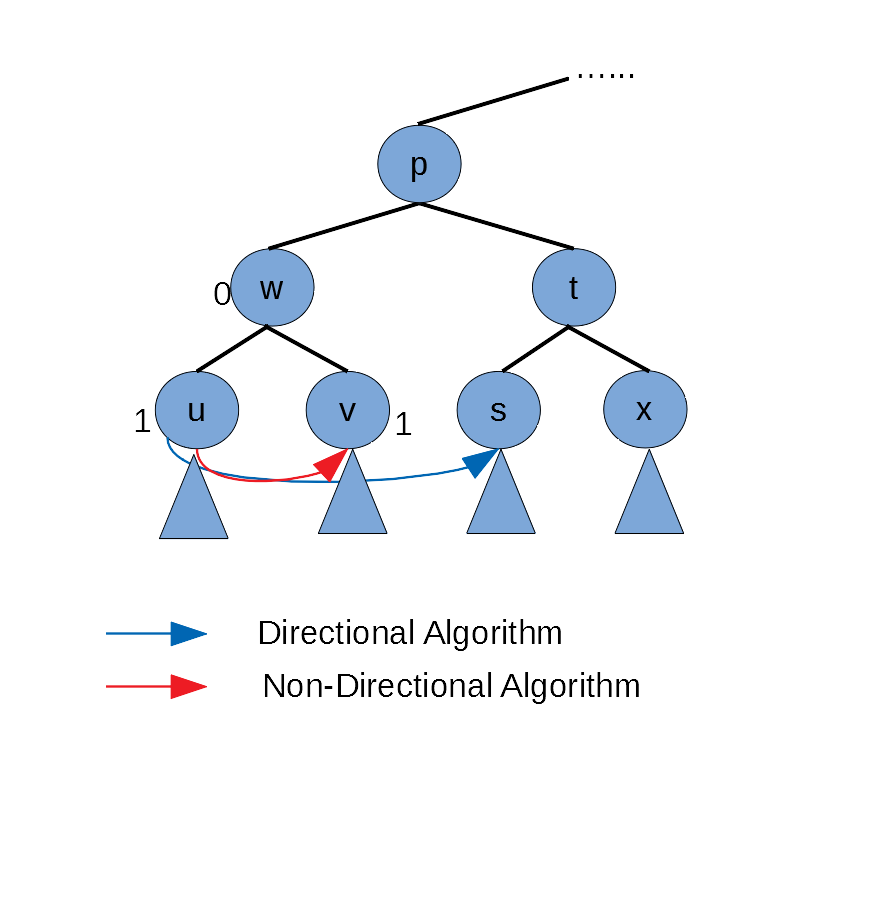
\includegraphics[width=0.7\linewidth]{nondir}
	\caption{ Non-Directional Algorithm case 1}
	\label{fig:nondir}
\end{figure}
\begin{proof}
	For case 1.If $u$ and $v$ are siblings, then the non-deterministic algorithm omits $v$ because it can determine the value of $w$ by visiting .Vertex $w$'s value could be determined only when $u$ is true and $w$ must be $false$. According to section 4, we already know that 
	this means $v$'s value could also been determined as false. Therefore, for any non-directional algorithm who evaluate $v$, the time for this process is wasted. 
	
	In conclusion, this case non-directional algorithm could not be faster than directional algorithm
\end{proof}

\subsection{Non-Directional Algorithm Case 2}
   In this case. $u$ and $v$ are not siblings, but their parents are siblings. Vertex $u$ could not determine the $w$'s value, but instead of visiting its sibling, non-directional algorithm 2 jumps out to visit $v$, who is in another sub tree. After visiting vertex $v$, there are two small cases: either jump back to visit $z$, or continue by visiting $y$. The non-directional algorithm 2 follows the figure below:
   \begin{figure}[H]
   	\centering
   	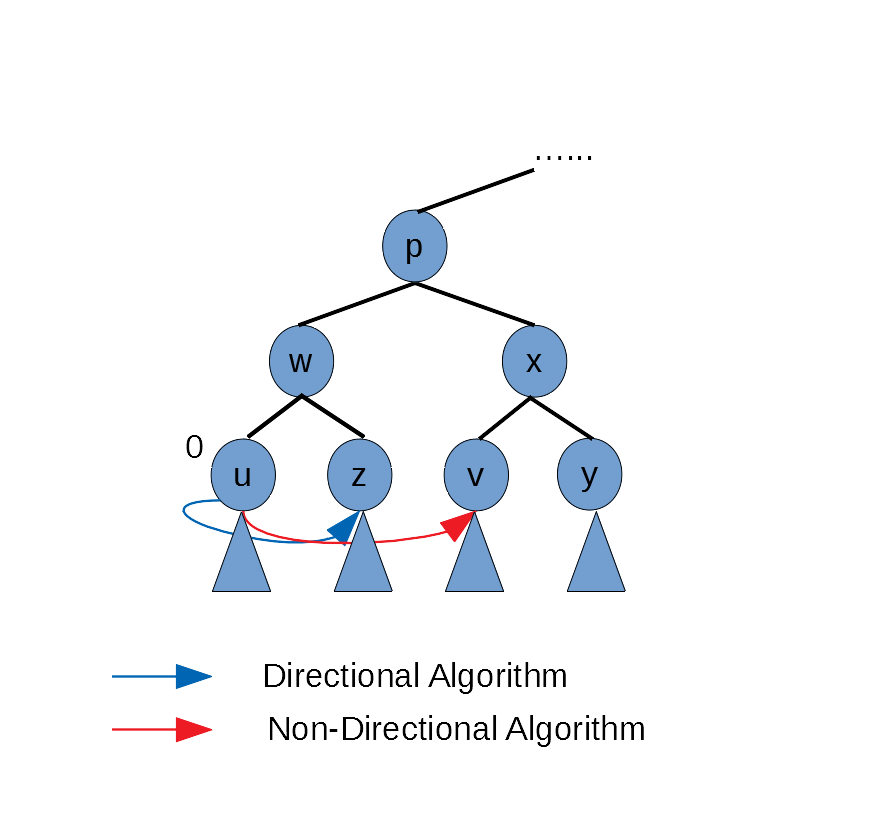
\includegraphics[width=0.7\linewidth]{nondir_case2}
   	\caption{Non-Directional Algorithm case 2}
   	\label{fig:nondircase2}
   \end{figure}

   If $u$ and $v$ are not siblings but at the same level, the non-directional algorithm 2 will visit $v$ when $w$'s value has not been determined. This non-directional algorithm will take advantage when only by visiting $v$ and its sibling could determine $p$'s value and z should be omitted. In this situation, $u$'s value should be 0, and $x$'s value should be 1. Therefore $v$ and its sibling $y$'s value should be 0, and $p$'s value should also be $0$.$z$ should be 1, because if $z$ is 0, then $p$'s value could be determined by directional algorithm by visiting $z$ after $u$, the visit of $u$ in non-directional algorithm is a waste. Let's prove it is also faster for trees of height n by induction. 
   
   Assumption: $E(c_N(x))$ depends only on the height of the tree rooted at $x$ and on the value of vertex $x$, but it does not depend on the state of the algorithm (for example, it is immaterial whether $x$ is the first or second child visited in the tree rooted at $x$'s parent). 
   
   E.g. $E(c_N(x)|w=1,x=0)$ actually does not include $E(c_N(u)|w=1,x=0)$, it just includes expectation of node $v$ and node $y$. This means though at this state of algorithm, of which we must evaluate vertex $u$ first before the evaluation process of vertex $x$, the expectation of evaluation cost of $x$ is not affected by the expectation of $u$. It should just determined by its own sub-trees' expectation. Otherwise we could say that, the expectation of a vertex is just determined by its own structure, but not by algorithm.
\begin{proof}       
   Assuming that directional algorithm is faster than or equal to non-directional algorithm for trees of height 1,2,...,n-1. For nor-tree of height n:
   Let $E(c(s))$ be the expected cost of an vertex $s$ in directional algorithm and $E(c_N(s))$ be the expected cost of an vertex $s$ in non-directional algorithm. Let $P,X,W$ be situation when $w=0,x=0$, $w=0,x=1$ and $w=1,x=0$
   The expected cost of directional algorithm is:
   \begin{equation}
   \begin{aligned}
   	E(c(p))=Pr[P]E[c(w)|P]+Pr[P]E[c(x)|P]+\\
   	Pr[X]E[c(w)|X]+Pr[X]E[c(x)|X]+Pr[W]E[c(w)|W]
   \end{aligned}
   \end{equation} 
   
   For the non-directional algorithm, there are two sub-cases. 
   If the algorithm continues to visit vertex $y$ before going back to $z$, then:
   \begin{equation}
   \begin{aligned}
     E(c_N(p))=Pr[P]E[c_N(w)|P]+Pr[P]E[c_N(x)|P]+Pr[X]E[c_N(u)|X]+\\
     Pr[X]E[c_N(x)|X]+Pr[W]E[c_N(w)|W]+Pr[W]E[c_N(x)|W]
   \end{aligned}
   \end{equation}
   	
   For jumping back to $z$'s case:
   \begin{equation}
   \begin{aligned}
   	E(c_N(p))=Pr[P]E[c_N(w)|P]+Pr[P]E[c_N(x)|P]+Pr[X]E[c_N(w)|X]+\\
   	Pr[X]E[c_N(x)|X]+Pr[W]E[c_N(w)|W]+Pr[W]E[c_N(v)|W]
   \end{aligned}
   \end{equation} 
   
   For the algorithm continues to visit vertex $y$:
   \begin{equation}
   	E(c_N(p))-E(c(p))\ge Pr[W]E[c_N(x)|W]-Pr[X]E[c(w)|X]+Pr[X]E[c_N(u)|X]
   \end{equation}
   Based on the assumption: $E[c_N(x)|W]=E[c_N(w)|X]$, which means that the expectation of $x$ under $W$ is equal to the expectation of $w$ under $X$, because the condition and value of these two are the same in these two different situation.
   For the algorithm jump back to visit $z$:
   \begin{equation}
   	E(c_N(p))-E(c(p))\ge Pr[W]E[c_N(v)|W]
   \end{equation}

   Thus we could find that directional algorithm is faster;
\end{proof}

\subsection{Non-Directional Algorithm Case 3}

In this case. $u$ and $v$ are not siblings, and they may not in the same height. Their parents are not siblings; Vertex $u$ could not determine the $w$'s value, but instead of visiting its sibling, non-directional algorithm 3 will jump out to visit $v$, who is in another sub tree and in different height. The non-directional algorithm 3 follows the figure below:
\begin{figure}[H]
	\centering
	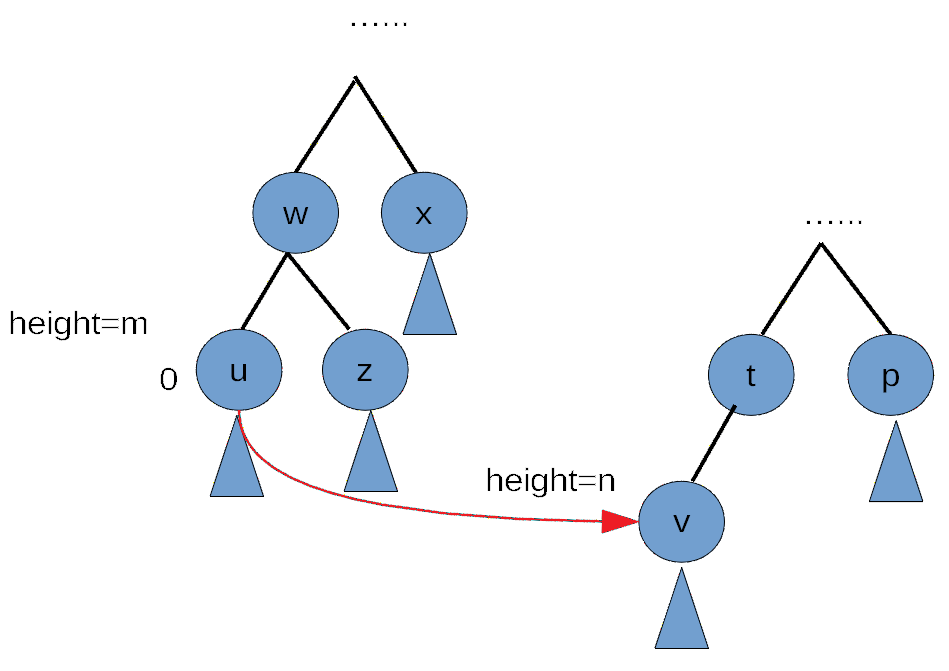
\includegraphics[width=0.5\linewidth]{nondir_case4}
	\caption{Non-Directional Algorithm case 3}
	\label{fig:nondircase4}
\end{figure}

	In this case, let$p$ be the nearest common parent of $u$ and $v$ and $w$ and $x$ be its child nodes.just as the figure below shows:
	\begin{figure}[H]
		\centering
		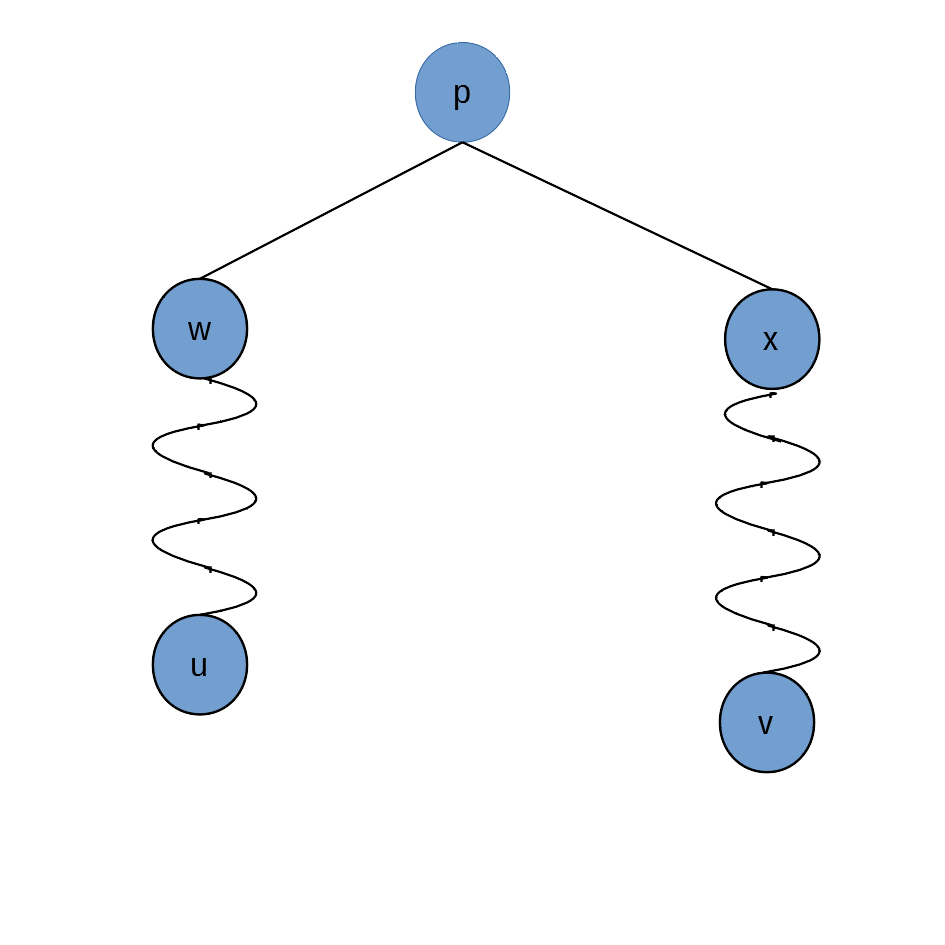
\includegraphics[width=0.5\linewidth]{nondir_case3def}
		\caption{Non-Directional Algorithm case 3 transform }
		\label{fig:nondircase3def}
	\end{figure}
	Similar to case 2's proof, we will prove this by induction. Assuming that directional algorithm is faster than or equal to non-directional algorithm for trees of height 1,2,...,n-1. For nor-tree of height n, Here are several small cases here:
	\begin{enumerate}
		\item The non-directional algorithm continue visit the sub tree containing $v$;
		\item The  non-directional algorithm jump back to $u$ to visit that sub tree.
		\item The non-directional algorithm jump to different subtrees randomly.
	\end{enumerate}
	
	\begin{proof}
		Let $P,X,W$ be situation when $w=0,x=0$, $w=0,x=1$ and $w=1,x=0$.et $E(c(s))$ be the expected cost of an vertex $s$ in directional algorithm and $E(c_N(s))$ be the expected cost of an vertex $s$ in non-directional algorithm.
		
		The expected cost of directional algorithm is:
		\begin{equation}
		\begin{split}
		    E(c(p))=Pr[P]E[c(w)|P]+Pr[P]E[c(x)|P]+Pr[X]E[c(w)|X] \\
		        +Pr[X]E[c(x)|X]+Pr[W]E[c(w)|W]
		\end{split}
		\end{equation}
		
		For non-directional algorithm continue visit the sub tree containing $v$:
		\begin{equation}
		\begin{split}
		   E(c_N(p))=Pr[P]E[c_N(w)|P]+Pr[P]E[c_N(x)|P]+Pr[X]E[c_N(u)|X] \\
		   +Pr[X]E[c_N(x)|X]+Pr[W]E[c_N(w)|W]+Pr[W]E[c_N(x)|W]
		\end{split}
		\end{equation}
		
		For non-directional algorithm jump back to $u$ to visit that sub tree:
		\begin{equation}
		\begin{split}
		E(c_N(p))=Pr[P]E[c_N(w)|P]+Pr[P]E[c_N(x)|P]+Pr[X]E[c_N(w)|X]\\
		+Pr[X]E[c_N(x)|X]+Pr[W]E[c_N(w)|W]+Pr[W]E[c_N(v)|W]
		\end{split}
		\end{equation}
		
		For the algorithm continue visit the sub tree containing $v$:
		\begin{equation}
		E(c_N(p))-E(c(p))\ge Pr[W]E[c_N(x)|W]-Pr[X]E[c(w)|X]+Pr[X]E[c_N(u)|X]
		\end{equation}
		
		Based on the assumption: $E[c_N(x)|W]=E[c_N(w)|X]$, the algorithm jump back to $u$ to visit that sub tree:
		$$E(c_N(p))-E(c(p))\ge Pr[W]E[c_N(v)|W]$$
		
		Therefore we could conclude that directional algorithm is faster than the non-directional one in this case.
	\end{proof}
	
	
	
	
%background
\chapter{Experiment and Analysis for Algorithm's Versatility}
From previous chapters, we have proved the algorithm in uniform binary tree. We wonder whether this evaluation process could still be useful in other types of binary trees. Therefore, in this section, we will analyze the game tree evaluation algorithm through two different types binary game tree, Fibonacci tree and skew-F tree. These experiments could help us to understand the Versatility for this algorithm.
\section{Fibonacci Tree}
\subsection{Definition}
Fibonacci tree\cite{FIBONACCI1982} is defined as a set of binary trees representing the recursive call structure of the Fibonacci computation process. It has n-1 internal nodes and n leaves. 
The root's value of Fibonacci tree is equal to the $n$th Fibonacci number. The left sub-tree should represent the computation process of $n-1$th
Fibonacci number, and the right sub-tree of root should represent the computation process of the $n-2$th Fibonacci. An Example of Fibonacci tree with height $4$ is shown below
     
\begin{figure}[H]
	\centering
	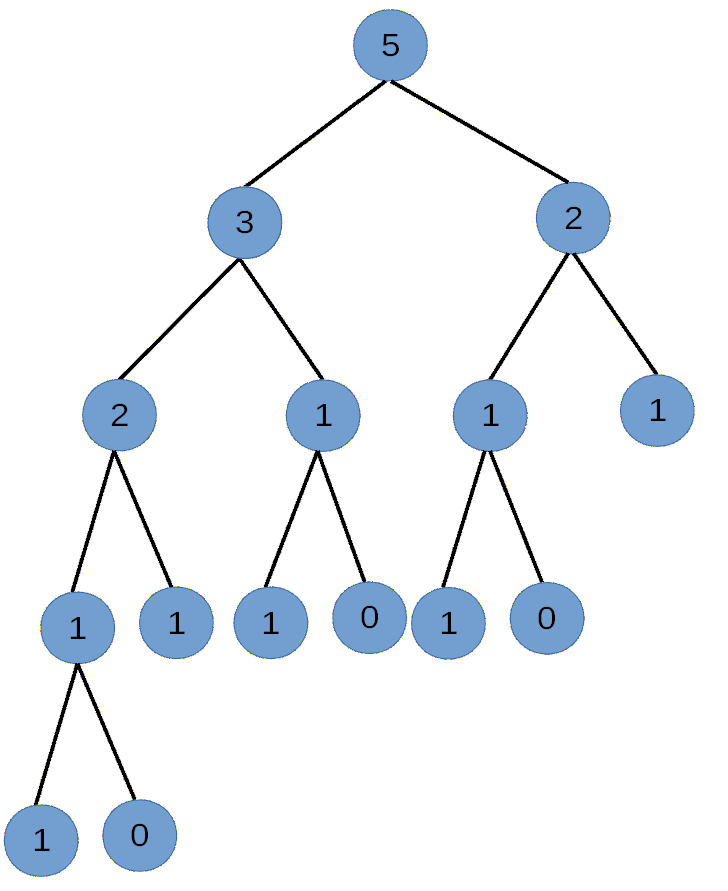
\includegraphics[width=0.5\linewidth]{fibo_tree}
	\caption{Fibonacci Tree}
	\label{fig:fibotree}
\end{figure}

\subsection{Fibonacci Tree Evaluation}
We will define a reluctant input, and let
$L(k, i)$ ($k = 0,1, 2, \dots$; $i = 0 ,1$) be 
the expected number of leaves visited by a deterministic
depth-first pruned algorithm for a Fibonacci tree of height $k$ which evaluates to true or false if $i = 1$ or $0$ respectively.
We first have that 
\begin{equation}
\label{eq:L1Fibonacci}
L(k, 1) = L(k-1, 0) + L(k-2, 0)
\end{equation}
\begin{equation}
L(0,x)=1(x=1,0)
\end{equation}


Let $p_k$ be defined recursively by $p_1 = 1/2$ and
$$\frac{p_k}{1 - p_{k}}=\frac{L(k-1,0)}{L(k-2,0)}$$.
The reluctant input is defined as follows.
If we wish that the $k$-th Fibonacci tree ($k > 0$) evaluates to 0,
then the input will make sure that at least one of the
subtrees evaluates to 0.
Specifically, the left subtree evaluates to 0 with probability $p_k$
and to 1 with probability $1 - p_k$.
Consequently, the right subtree evaluates to 0 with probability $1 - p_k$
and to 1 with probability $p_k$.


Consider first a directional algorithm that chooses
to descend to the left subtree. Its expected cost is:
$p_k L(k-1,1) + (1 - p_k)[L(k-1,0)+L(k-2,1)]$.
If instead the directional algorithm chooses to descend to the right
subtree, then its expected cost is
$(1 - p_k) L(k-2,1) + p_k [L(k-2,0) + L(k-1,1)]$, 
which by the choice of $p_k$ is the same as the cost of the algorithm
that descended to the left.

Hence, by using \eqref{eq:L1Fibonacci}, we have that
\begin{equation}
\label{eq:L0Fibonacci}
L(k,0) = p_k L(k-2,0) + (1 - p_k) L(k-1,0) + L(k-3,0) + (1-p_k) L(k-4,0)\;
\end{equation}

\iffalse
Define the sequence $\rho_k$ as the solution to the recurrence:
which could transfer to:

\begin{equation}
\rho_ka^k = \frac{a}{1+a}\rho_{k-2}a^{k-2}+\frac{1}{a+1}\rho_{k-1}a^{k-1}+\rho_{k-3}a^{k-3}+\frac{1}{a+1}\rho_{k-4}a^{k-4}
\end{equation}
\fi

Define the sequence $\rho_{k}$ as the solution to the $L(k,0)$ recurrence:
\begin{flalign}
\label{eq:Fiborhokrecursive} \rho_k &=  \frac{\rho_{k-1}}{a^2+a} +  \frac{\rho_{k-2}}{a^2+a} + \frac{\rho_{k-3}}{a^3} + \frac{\rho_{k-4}}{a^5+a^4}\\
\label{eq:Fiborhok4}         \rho_4 &= \frac{6.558171076}{a^4}\\
\label{eq:Fiborhok3}         \rho_3 &= \frac{4.512036108}{a^3}\\
\label{eq:Fiborhok2}         \rho_2 &= \frac{3.189189189}{a^2}\\
\label{eq:Fiborhok1}         \rho_1 &= \frac{2.2}{a} 
\end{flalign}

Define  
\begin{equation}
\label{eqn:L0fiboRecur} L(k,0) = \rho_k a^k
\end{equation} and $r_k$ as the recurrence vector of $\rho_{k}$
\begin{alignat*}{2}
\vect{r}_{k} & = 
\begin{pmatrix}
\rho_{k+3} \\
\rho_{k+2} \\
\rho_{k+1} \\
\rho_{k}
\end{pmatrix} &\qquad&
(k = 1, \dots )
\end{alignat*}


Then we have $\vect{r}_k=A\vect{r}_{k-1}$, where 

\begin{equation}
A = 
\begin{pmatrix}
\frac{1}{a+a^2} & \frac{1}{a+a^2} & \frac{1}{a^3} & \frac{1}{a^4+a^5}  \\
1               & 0               & 0             & 0                  \\
0               & 1               & 0             & 0                   \\
0               & 0               & 1             & 0                   \\
\end{pmatrix}\;
\end{equation}

The characteristic equation is:
\begin{equation}
\det(A-\lambda I)=\det\left(\begin{pmatrix}
\frac{1}{a+a^2} - \lambda & \frac{1}{a+a^2} & \frac{1}{a^3} &                \frac{1}{a^4+a^5}                                                \\
1               & -\lambda        & 0             & 0             \\
0               & 1               & -\lambda      & 0             \\
0               & 0               & 1             & -\lambda       \\
\end{pmatrix}\right)\;
=0
\end{equation}
which solved for $\lambda$ gets the claimed eigenvalues with
\begin{equation}
\lambda^4-\frac{\lambda^3}{a+a^2}-\frac{\lambda^2}{a+a^2}-\frac{\lambda}{a^3}-\frac{1}{a^4+a^5} = 0
\end{equation}

For $a$, with:
\begin{equation}
A \vect{v}_1 = \vect{v}_1
\end{equation}
where $\vect{v}_1$ is\footnote{This is not the vector that you use later on}
$$\begin{pmatrix}
1 \\
1 \\
1 \\
1
\end{pmatrix}\;$$
We could get:
$$ a^5 + a^4 -2 a^3 -a^2 -a -1=0 $$
Let a = $1.439650182$. 
We could get:
$$ \lambda^4 -0.284718354857539 \lambda^3 -0.095421125796929-0.335142164770774 \lambda -0.284718354857539 \lambda^2 = 0$$
whose root is:
$$\begin{pmatrix}
1.000000000 \\
-0.313238282 \\
- 0.201021681 + 0.514021596i \\
- 0.201021681 - 0.514021596i
\end{pmatrix}\;$$

We could see that the eigenvalues of A are $\lambda_1 = 1$ and other eigenvalues($\lambda_2, \lambda_3, \lambda_4$) with real part less than 0. Therefore $\vect{r}_k$ tends to the projection of $\vect{r}_1$ along an eigenvector $\vect{v}_1$ corresponding to $\lambda_1$. By using the corresponding eigenvectors to find the component r of $\vect{r}_1$ along $\vect{v}_1$, we could prove the claim. 
We could get $\vect{r}_1$ is:
\begin{alignat*}{2}
\vect{r}_{1} & = 
\begin{pmatrix}
\rho_{4} \\
\rho_{3} \\
\rho_{2} \\
\rho_{1}
\end{pmatrix} 
\end{alignat*}
By relationship:
$$\begin{pmatrix}
\vect{v}_1 & \vect{v}_2 & \vect{v}_3 & \vect{v}_4  
\end{pmatrix} 
\begin{pmatrix}
r\\
s\\
t\\
u   
\end{pmatrix} = 
\begin{pmatrix}
\rho_1\\
\rho_2\\
\rho_3\\
\rho_4
\end{pmatrix}
$$ 

We could get $r = -3.052885190463789$. Since $lim_{k\rightarrow\infty}r_k=r\vect{v}_1$ We have that
\begin{equation}
lim_{k\rightarrow\infty}\rho_{k}=-0.5r=1.52644259523189
\end{equation}

\begin{lemma}
	\label{lemma:rhok_Fibo}
	$L(k,0)$ is bounded by $L(k,0)=\rho_{k}a^k$
\end{lemma}

\begin{proof}
	Define for convenience of notation $T(k) = L(k, 0)$.
	By \eqref{eqn:L0fiboRecur} , 
	we have that $T(1) = \rho_1 a, T(2)=\rho_{2}a^2, T(3) = \rho_{3}a^3, T(4)=\rho_{4}a^4$.
	By induction process, \eqref{eq:L0Fibonacci}, and definition \eqref{eq:Fiborhokrecursive} we have $T(k)=\frac{a^{k-1}}{a+1}\rho_{k-1}+\frac{a^{k-1}}{a+1}\rho_{k-2}+a^{k-3}\rho_{k-3}+\frac{a^{k-4}}{a+1}\rho_{k-4}$, which completes the proof.
\end{proof}

By combining the lemma and recurrence relationship
we obtain the following tighter lower bound:

\begin{theorem}
	We have that 
	$\lim_{k \rightarrow \infty} L(k, 0) / a^{k} = \rho $
	and
	$\lim_{k \rightarrow \infty} L(k, 1) / a^{k-2} = (a+1)\rho$.
\end{theorem}

\section{skew F-tree}
\subsection{Definition}
A skew F-tree $S^k$is a NOR tree defined inductively: $S^k$ is a single vertex, and for every specific vertex $S^n$ in higher level will have left sub-tree as a single vertex, and right sub tree $S^{n-1}$.\citep{PROBABILISTIC}

\begin{figure}[H]
	\centering
	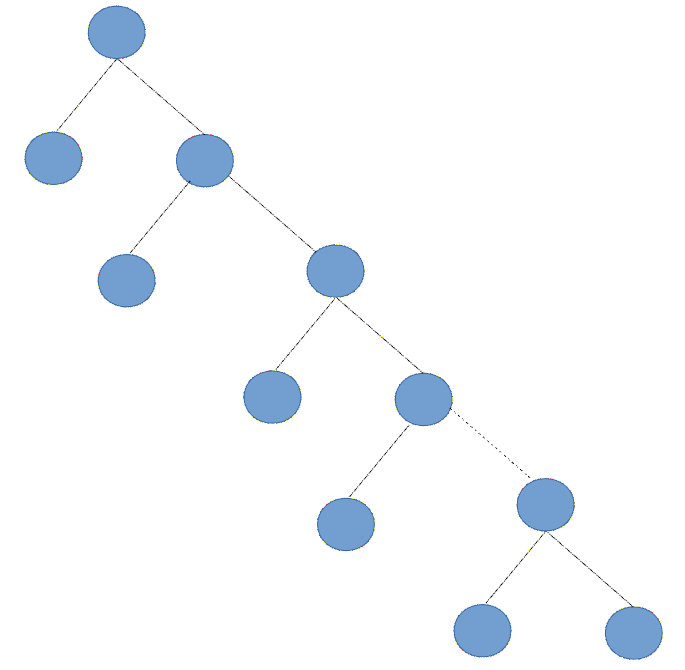
\includegraphics[width=0.5\linewidth]{skew}
	\caption{skew-F tree Example}
	\label{fig:skew}
\end{figure}

\subsection{Evaluation of skew F-tree}
From the definition in the last section, it is clear that:
\begin{flalign}
\label{eqn:skewL1} L(k, 1) &= L(k-1,0)+1\\
\label{eqn:skewLbase} L(0,i) &= 1 \quad (i = 0,1)
\end{flalign}
and also that $L(k,1) \leq k + 1$.
The reluctant input is defined as follows.
If we wish that the $k$-th Skew-F tree ($k > 0$) evaluates to 0,
then the input will make sure that at least one of the
subtrees evaluates to 0.
Specifically, the left subtree evaluates to 0 with probability $p_k$
and to 1 with probability $1 - p_k$.
Consequently, the right subtree evaluates to 0 with probability $1 - p_k$
and to 1 with probability $p_k$.
\begin{flalign}
\label{eqn:detskewL0a} L(k, 0) &= p_k+(1-p_k)(L(k-1,1)+1)\\
\label{eqn:detskewL0b} L(k, 0) &= p_k(L(k-1,0)+1)+(1-p_k)L(k-1,1)
\end{flalign}
Therefore we could have:
\begin{equation}
\label{eq:pkL0skew}p_k = \frac{1}{1 + L(k-1,0)} = \frac{1}{L(k, 1)}
\end{equation}


Consider first a directional algorithm that chooses
to descend to the left subtree. Its expected cost is \eqref{eqn:detskewL0a}
If instead the directional algorithm chooses to descend to the right
subtree, then its expected cost is
\eqref{eqn:detskewL0b} 
which by the choice of $p_k$ is the same as the cost of the algorithm
that descended to the left.

Therefore, by using \eqref{eq:pkL0skew} and \eqref{eqn:skewL1}, we could get:
\begin{flalign}
\label{eqn:skewRecur} L(k,0)=\frac{L(k-1,0)L(k-2,0)+2L(k-1,0)+1}{1+L(k-1,0)}\\
\label{eqn:skewRecur1}
L(k,1)=L(k-2,1) - \frac{L(k-2,1)}{L(k-1,1)}+2
\end{flalign}

Then we will show that $L(k,1) \ge \frac{k}{2}$ by induction:
\begin{proof}
	We start an induction with:
	\begin{flalign}
	\label{sft01}L(0,1) = 1\\
	\label{sft11}L(1,1) = 2\\
	\label{sft21}L(2,1) = 2.5\\
	\label{sft31}L(3,1) = 3.25
	\end{flalign}
	Ee could see that $L(k,1) \ge \frac{k}{2}$ stands in base condition.
	With \eqref{eq:pkL0skew}, we know that when $L(k,1)$ becomes large enough, we could say $pk = 0$. 
	Considering $L(k,0)$ when $k$ is even and large enough so we could consider $p_k$ as 0, we could have:
	\begin{flalign}
	\label{sftlbk0}L(k,0) = L(k-1,1)\\
	\label{sft1bkm11}L(k-1,1) = 1+L(k-2,0)
	\end{flalign}
	Then we could have $L(k,0) = \frac{k+1}{2}$ and $L(k,1)\ge\frac{k}{2}+1$. 
\end{proof}

In conclusion, for skew-F tree, $\frac{k}{2}+1 \le L(k,1)\le k+1$.

\subsection{conclusion}
From these two experiments, we have showed that this game tree evaluation algorithm could also be used for evaluating other types game tree for getting their lower bounds. Many other types of binary game tree could also be tested, but as the whole method is fixed, and we could prove it by Yao's principle. Therefore we could say that this game tree evaluation analysis process has versatility.
\chapter{Conclusion and Future Work}

In this chapter, we will discuss some of the strengths and weaknesses of the new game tree evaluation process, and also describe some methods for future work.

All in all, we believe that we have proposed an algorithm for evaluating uniform binary game tree with comparison in Chapter 4 and Chapter 5. We have made very detailed calculation for both directional and Non-directional algorithm's lower bound and prove it with iteration. We have shown this method could also be used for evaluating some more complex type binary game trees but not only uniform tree, including Fibonacci tree, skew-F tree. 

One important strength of our analysis is trying to find out the best probability distribution at first and tighter the lower bound by including conditional probability. This helps us get the better lower bound than "Randomized Algorithm".

In short, we have constructed an algorithm with better lower bound compared with classical game tree evaluation steps which could be used for many cases of binary game tree evaluation.

One important weakness of this algorithm is from the analysis it self. We made some limitation in analysis, which may lead to some loose for the final lower bound result. A tighter lower bound still could be found. Also this algorithm only could be applied for binary game tree. It is questionable its usage in ternary and other types of game tree. In addition, although we already know it is more efficient in binary game tree, we don't know whether this is still good enough in other cases.

Therefore it is clear that there are some future work needed to be done for this algorithm. First of all, this evaluation process only been demonstrated in binary game tree. It is clear that there are many other types of a game trees, like ternary tree, quad tree, or some realistic game tree like the tic-tac-toe game tree, chess board game tree. A more general algorithm may be needed to propose for game tree evaluation based on the previous method, which may includes the number of nodes in each level, different type of boolean functions and so on. Then the algorithm could be applied for many different cases. 

Then it is clear that most of the experiments and analysis are for theatrical field. We could not figure out how this promotion of algorithm could be used for some practical environment. this also could be an important part for the future work. Combined with the a more general evaluation algorithm, some cool things maybe done. For example maybe we could use this analysis method for realistic chess game cases, and calculate the probability to win for both of the two players.

Last but not least, although our algorithm is good enough for game tree evaluation, most of its method is based and inspired by the methods that already known. Obviously, if we could find some new approach that is totally unknown and different from the past will be a very cool thing. 

In conclusion. A more efficient approach for binary game tree evaluation has been proposed by us. It has better lower bound and could be used for evaluates different types of binary game tree. Considering its weakness of using for non-binary game tree, the future work should focus on improve this method for more types of game tree. If possible try its usage in some practical filed like board game will be good. In theoretical aspect, to discover a totally new approach different from previous will be a good method.


%\include{10-Summary}
\appendix
\chapter{Detailed Calculation}
\subsection{Lemma \ref{lemma:rhok}}
The characteristic equation is:
\begin{equation}
A-\lambda I=\begin{pmatrix}
\frac{1}{2 a}-\lambda & \frac{2}{a^2} \\
1             & -\lambda 
\end{pmatrix}\;
=\lambda^2-\frac{1}{2 a}\lambda-\frac{2}{a^2}=0
\end{equation}
which solved for $\lambda$ gets the claimed eigenvalues.

We know that $\vect{v}_1 = A \vect{v}_1  $, which is:
\begin{equation}
\begin{pmatrix}
x \\ 
y 
\end{pmatrix}\;
=
\begin{pmatrix}
\frac{1}{2 a} & \frac{2}{a^2} \\
1             & 0 
\end{pmatrix}\;
\begin{pmatrix}
x \\ 
y 
\end{pmatrix}\;
\end{equation}
By calculation:
\begin{flalign}
\label{eqn:xany}x &= \frac{1}{2 a}x+\frac{2}{a^2}y\\
\label{eqn:xey} y &= x
\end{flalign}
By \eqref{eqn:xany}, we could find $x$ could be any value. 
We already know that $\vect{v}_1$ is a unit vector.

Because $A \vect{v}_2 = \lambda_2 \vect{v}_2$. Thus we could find:
\begin{equation}
\lambda_2
\begin{pmatrix}
x \\ 
y 
\end{pmatrix}\;
= 
\begin{pmatrix}
\frac{1}{2 a} & \frac{2}{a^2} \\
1             & 0 
\end{pmatrix}\;
\begin{pmatrix}
x \\ 
y 
\end{pmatrix}\;
\end{equation}
By calculation, 
\begin{flalign}
\label{eqn:xany2}\lambda_2 x &= \frac{1}{2 a}x+\frac{2}{a^2}y\\
\label{eqn:x2ey}\lambda_2 y &=  x
\end{flalign}
Therefore we could get:
$$\vect{v}_2 = 
\frac{1}{\sqrt{\lambda_2^2+1}}
\begin{pmatrix}
\lambda_2\\
1
\end{pmatrix}$$

The system of equation becomes:
$$\frac{\sqrt{2}}{2}\rho+\frac{\lambda_2}{\sqrt{1+\lambda_2^2}}\alpha = \rho_2 $$
$$\frac{\sqrt{2}}{2}\rho\lambda_2+\frac{\lambda_2}{\sqrt{1+\lambda_2^2}}\alpha = \rho_1\lambda_2$$
and subtracting the second equation from the first:
$$\rho=\frac{\rho_1\lambda_2-\rho_2}{\frac{\sqrt{2}}{2}(\lambda_2-1)}=\frac{40+8\sqrt{33}}{\sqrt{66}+33\sqrt{2}}\approx1.5687$$

\subsection{Lower Bound Comparison}
Since
$$\rho = \frac{20 \sqrt{2} + 4 \sqrt{66}}{\sqrt{66} + 33 \sqrt{2}}\;,$$
$$a = (1 + \sqrt{33}) / 4\;,$$
and the previous lower bound is $(2-p)^k$ where $p = (3-\sqrt{5})/2$. 
Then,
$$\lim_{k \rightarrow \infty} \frac{\rho\alpha^k}{(2 - p)^k} = \infty\;,$$
which implies that the new lower bound is strictly tighter than the previous one.

 % HHP profile

% To have a bibliography for the whole document, plus individual bibs,
% put \bibliography commands in the included chapters plus in the root
% file; use \usepackage[rootbib]{chapterbib}; run LaTeX; run BibTeX on
% the root file; change to \usepackage{chapterbib}; run LaTeX; run
% BibTeX on each included file; run LaTeX; run LaTeX. An `overall'
% bibliography only makes sense for various `named' bibliography
% styles; a style with numbering will give separate and unrelated
% numbers in each bibliography.
\renewcommand{\bibname}{Complete References}
\bibliographystyle{unsrt} %if you have problems with the style, consult the CWRU-thesis.cls file
\markright{\textit{Bibliography}}
%\renewcommand{\chaptername}{}
\bibliography{refs/my_references}
%if latex throws errors with the .bbl file, fix the problem in the .bib, and delete the .bbl before trying to recompile
%also, if the tex runs but says bib?, you can hit enter and get everything but the bibliography

%\end{document}
%\end


%%% Local Variables: 
%%% mode: tex-pdf
%%% TeX-master: t
%%% End: 


%\documentclass{article}
%\usepackage{units} %For use of \nicefrac{}{} to create units
%\usepackage{fixltx2e} %For use of \textsubscript{}

%%To widen the text columns from the default 'article' settings:
%\setlength{\hoffset}{25pt}
%\setlength{\marginparwidth}{0pt}
%\setlength{\oddsidemargin}{0pt}
%\setlength{\textwidth}{400pt}

%\begin{document}

%\title{Acrylic Durability for Long-Lived Low-Cost PV Systems}
%\author{Myles Murray}
%\maketitle
%\newpage
%\tableofcontents
%\newpage 
%


%\enddocument
\end{document}

				


